%%%%%%%%%%%%%%%%%%%%%%%%%%%%%%%%%%%%%%%%%%%%%%%%%%%%%%
\section{Introduction To The Standard Model}\label{secSM}



"Theorists can be wrong; only nature is always right" - David Gross\newline

%"Fortunately, nature is as generous with its problems as Nobel with his fortune. The more we know, the more aware we are of what we know not."- David Gross 


The Standard Model (SM) of particle physics is a quantum field theory (QFT) description of the strong, weak and electromagnetic forces of nature. The known particles of the SM are; 1 scalar Higgs boson,4 guage bosons, 6 types of quark, and 6 types of lepton. 

The quarks and leptons, particles which constitute matter, are fermions, obeying Fermi-Dirac statistics due to their half-integer spin. In contrast,the bosons have integer spin and obey Bose-Einstein statistics. Gauge bosons mediate the 3 fundamental forces and the Higg's boson is responsible for the electro-weak symmetry breaking which gives mass to the other particles\cite{Griffiths:111880}. 

The fermions are arranged into 3 generations, arranged in columns from left to right on \cite{fig:SM}



Quantum Chromodynamics, QCD, is the theory of the strong interaction which governs the interactions of quarks and gluons\cite{Griffiths:111880}.


The SM constitues humanity's most rigorous theory of our universe, providing predictions of observables which have since been measured, in the case of Quantum Electrodynamics, QED, to the highest precision of any scientific theory. Despite the impressive predictions,the gravitational force and more subtle phenomena, such as flavor oscillation of neutrinos \cite{Ashie:2005ik}, indicate the existence of physics beyond the standard model, BSM.

Various attempts have been made to unify the fundamental forces under one theory, thusfar the electromagnetic and weak interactions have been united by electro-weak theory. 

The Standard electroweak model can be described $SU(2) x U(1)$ mathematically.

The  $SU(2) x U(1)$ guage group is a convolution ( $<- $That is not the right word...) of the special unitary symmetry group $SU(2)$ describing 3 mixed massive vector bosons, $W_{-}$ $W_{+}$ $Z_0$, carriers of the weak nuclear force and the unitary gauge group $U(1)$ , describing the lonely massless chargeless photon, of the electromagnetic interaction.

The standard model of the strong interaction is known as quatum chromodynamics, QCD, a non-Abelian guage theory described by the special unitary group $(SU(3)_f)$, where the  flavours of quark are the physical manifestation of the symmetry group. This force is mediated by the 8 massless gluons which carry color charge, making QCD more complicated mathematically than QED.

The SM also contains a Higgs boson, an excitation of a scalar Higg's field, which gives rise to spantaneous symmetry breaking of the electroweak theory, providing the particles with mass, but I won't get into that. 

The quarks and leptons are arranged in generations according to their relative masses, as shown in Figure \ref{fig:SM}. The table also shows the spins of the particles, the leptons and quarks have half-integer spin, fermions, that obey the fermi exclusion principle, conversely the bosons have half integer spin and therefore obey bose-einstein statitics. Through the SM we interpret the observed hadronic particles, mesons ( baryons ) , as 2 quark (3 quark) bound states. The existence of spin $\frac{3}{2}$ baryons, which are symmetric bound states in space, spin and flavour and the need to obey Fermi-Dirac statistics, by maintaining total assymmetry of the wavefunction,implies there is another degree of freedom, called color, so that each quark is either red, green or blue. Granted only color singlet, containing either all 3 or 1 and it's anti color, states exist. Furthermore there exists a property of asymptotic freedom where the QCD coupling between quarks and gluons increases as they asymptotically approach one another. There exists a wealth of experiemental data to support the concept of asymptotic freedom despite the fact that rigorous mathematical proof of the exlusion of free quark and gluon states has yet to be acheived.


%image CMS:2014mna
% visuals/strong-coupling-cms


\begin{figure}[htb]
\centering
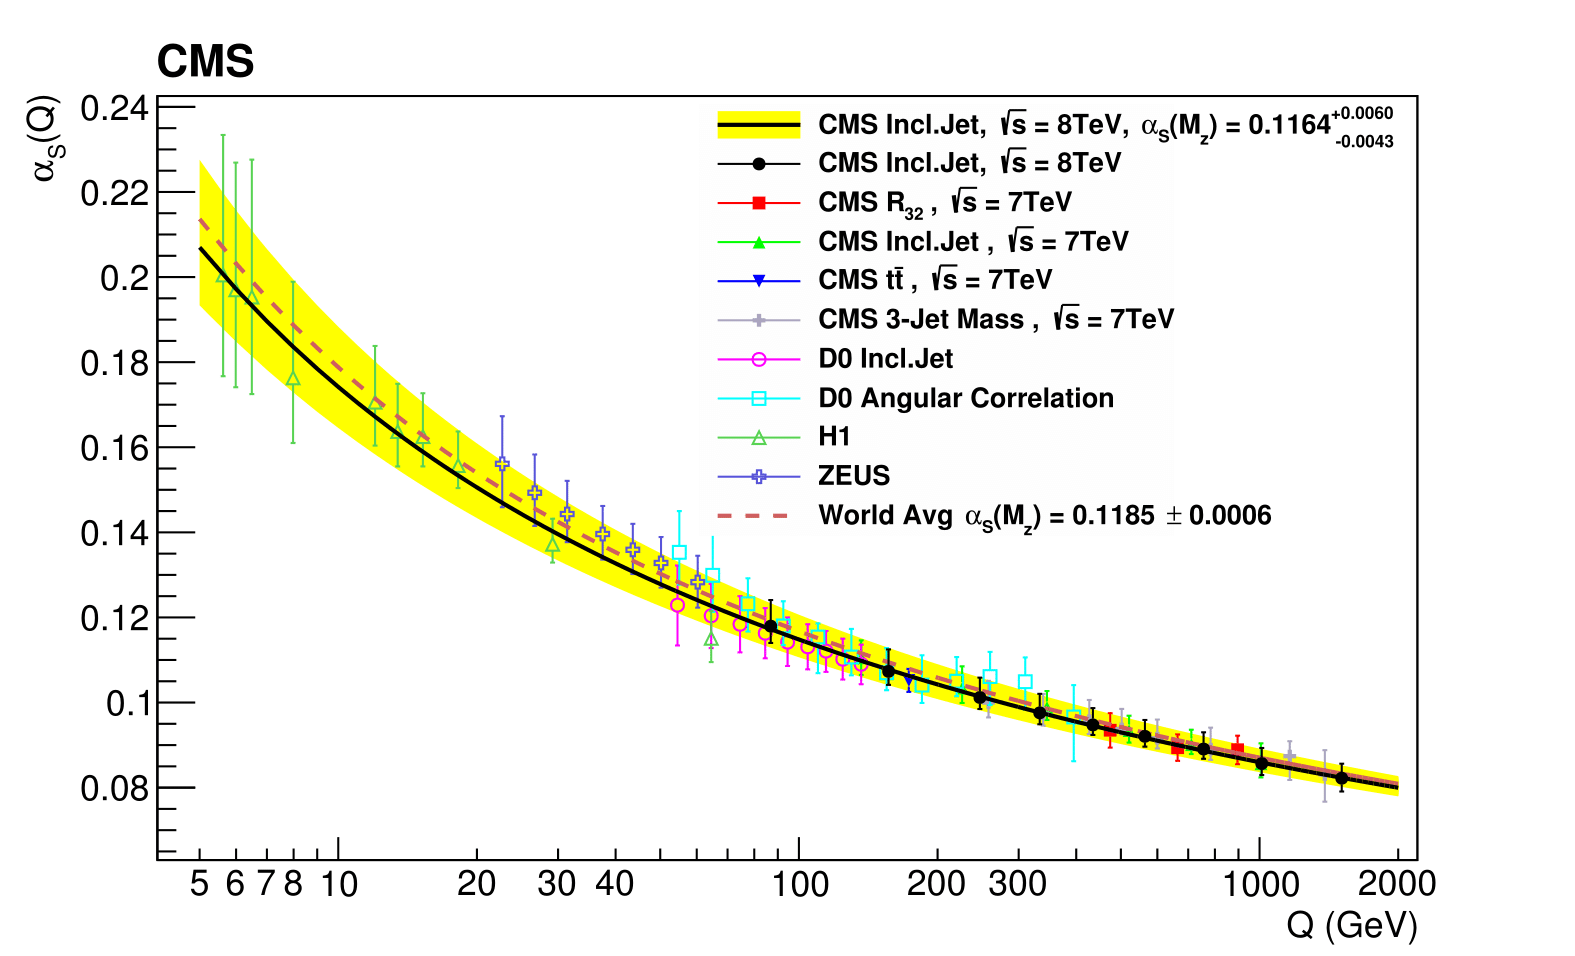
\includegraphics[width=1.0\textwidth]{visuals/strong-coupling-cms2.png}
\caption{The running of the strong coupling constand as compiled by CMS including measurements from CMS and HERA among others~\cite{CMS:2014mna}.}
\label{fig:alphas}
\end{figure}





%another DY thesis  http://inspirehep.net/record/1345977/files/DoolingSamantha_Dissertation.pdf

Assymptotic freedom is a useful property as it allows for perturbative calculations of QCD observables, this is discussed in section XXX.

% Symmetris imply conserved quantities, Neuther's Theorem

 Nuclei in ordinary matter are composed solely of $1^{st}$ generation particles, up and down quarks, bound by gluons. Neutral atoms contain an equal number of protons (composed of 2 up quarks and a down quark) and electrons, $1^{st}$ generation leptons. The main distinction between leptons and quarks, both fermions (particles of $\frac{1}{2}$ integer spin), being that leptons do not experience the color interaction $(SU(3)_f)$ like their quark friends. In each generation there is a quark with charge $Q = + \frac{2}{3}$ (up, charm, top) and another of charge $Q = - \frac{1}{3}$ (down, strange, bottom).



\begin{figure}[htb]
\centering
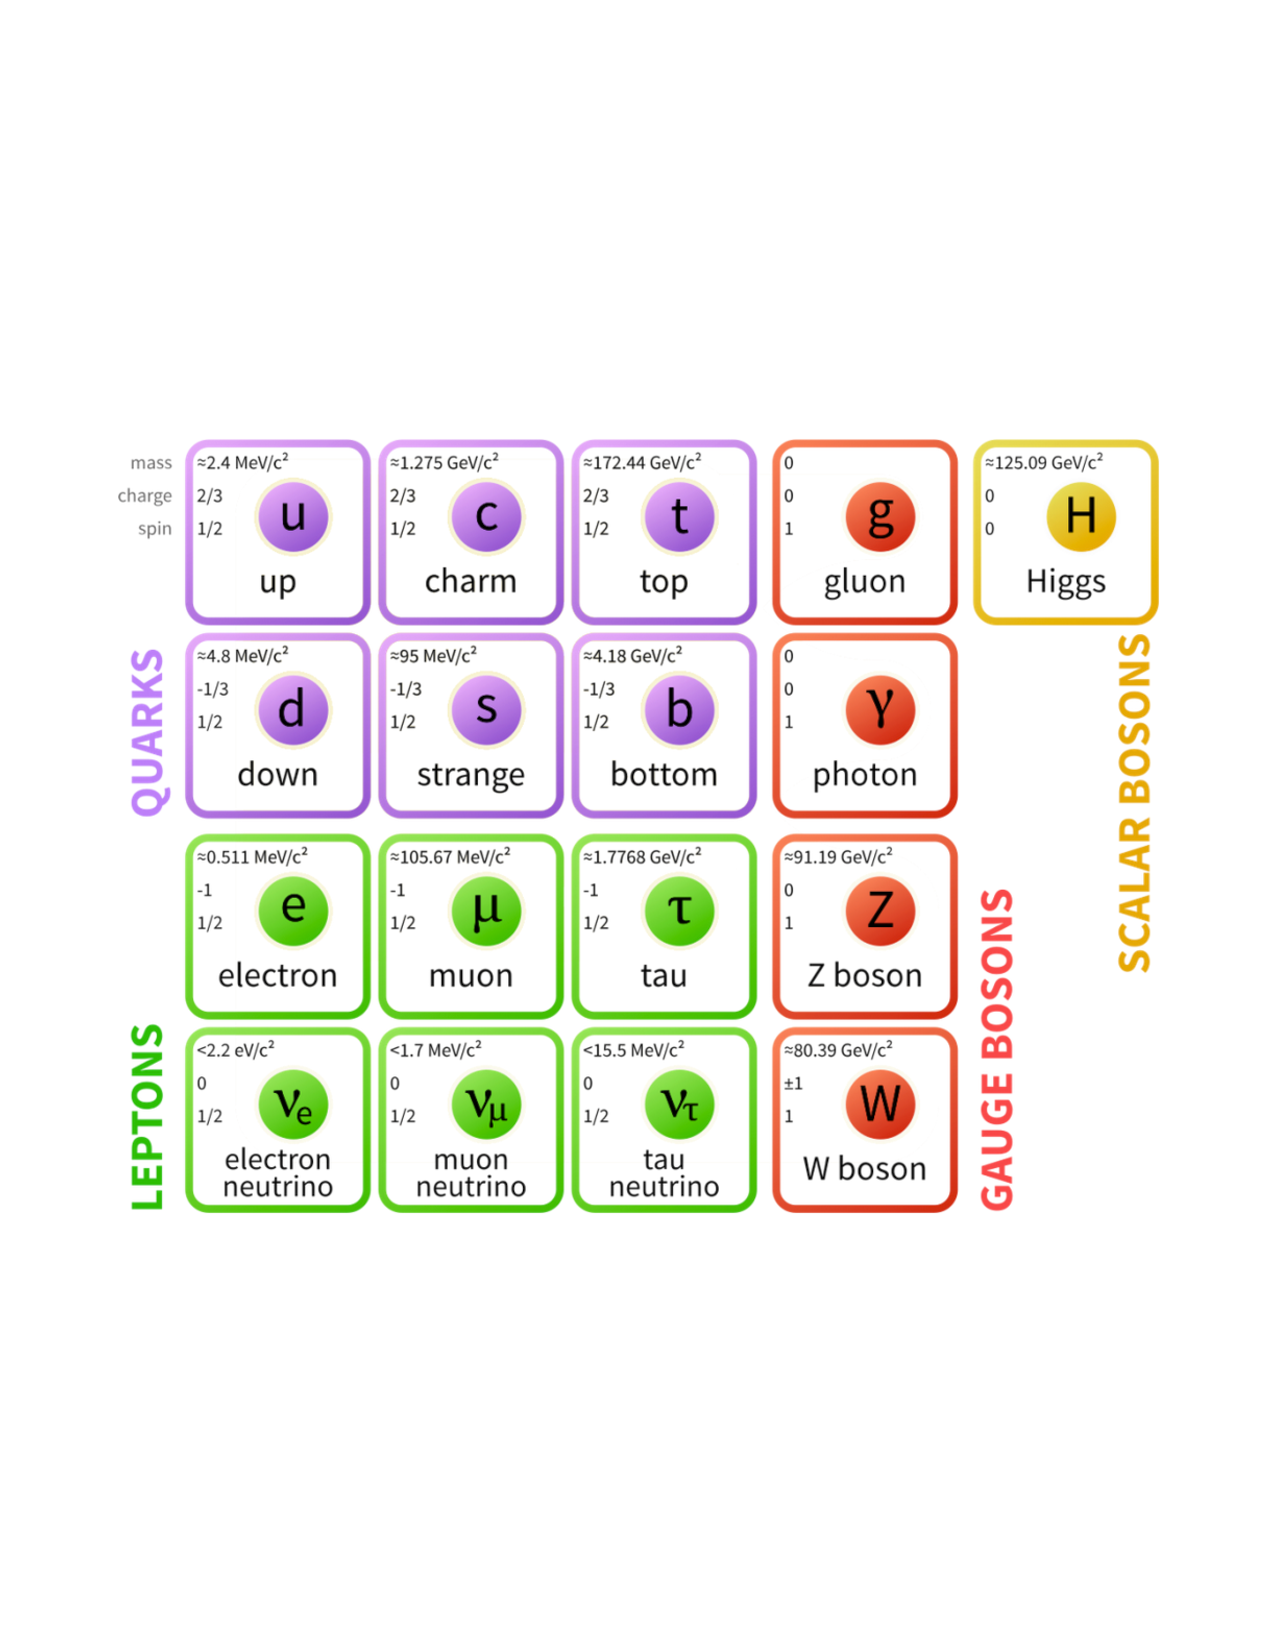
\includegraphics[width=1.0\textwidth]{smdiagram.pdf}
\caption{Fundamental particles of the Standard Model~\cite{modellinginvisible}.}
\label{fig:SM}
\end{figure}


\subsection{Quantum Electrodynamics}\label{secQED}





\subsection{Quantum Chromodynamics}\label{secQCD}


lagrangian

\begin{equation}
\mathcal{L}=-\frac{1}{4} F_{\mu \nu}^{A} F_{A}^{\mu \nu}+\sum_{\text {flavours }} \overline{\psi}_{a}\left(i \gamma_{\mu} D^{\mu}-m\right)_{a b} \psi_{b}
\end{equation}

\begin{equation}
F_{\mu \nu}^{A}=\partial_{\mu} A_{\nu}^{A}-\partial_{\nu} A_{\mu}^{A}+g_{s} f^{A B C} A_{\mu}^{B} A_{\nu}^{C}
\end{equation}

covariant derivative
\begin{equation}
\left(D_{\mu}\right)_{a b}=\partial_{\mu} \delta_{a b}-i g_{s} A_{\mu}^{A} t_{a b}^{A}
\end{equation}

In order to emphasize the relevance to the measurement presented herein, the theory of Quantum Chromodynamics is discussed here from a kinematic (<- better word?) rather than Lagrangian perspective. This is useful as jet studies help probe QCD in the soft and collinear limits. 
% https://arxiv.org/pdf/1709.06195.pdf CITE THIS LECTURE
Jets are formed by the hadronization of quarks and gluons. In this thesis I present a measurement of a light quark enriched jet sample. 



Consider the simplest process that could produce a quark initiated jet, a quark of energy $E_q$  emitting a gluon of energy $E_g$. The probability that this will occur is a function of the gluon's energy fraction, $z$, and the emission angle , $\theta$  \cite{Larkoski:2017fip}.\newline


$z = \frac{E_g}{E_q + E_g}$\newline

$1 - cos \theta = \frac{m^2}{2 E_q E_g}$\newline

Then the probability of gluon emission from the quark is :


$P_q(z,cos \theta) dz d cos \theta = \frac{\alpha_s C_F}{\pi}  \frac{dz}{z} \frac{dcos \theta}{1 - cos \theta}  $\newline

It is useful to assume the small angle approximation, $\theta << 1$, giving:\newline


$P_q(z,\theta^2) dz d \theta^2 = \frac{\alpha_s C_F}{\pi}  \frac{dz}{z} \frac{d \theta^2}{ \theta^2}  $\newline

Notice that the probability of emission diverges for very soft (small z) or very collinear (small $\theta$) gluons. In the soft and collinear limits the probability can be interpretted as an expectation value for the number of soft/collinear gluons \cite{Larkoski:2017fip}.

It is elucidating to rewite the probability in terms of inverse logarithms in the and intruduce the "Lund Diagram" in order to visualize the uniform distribution of soft and collinear gluons in the $log \frac{1}{ \theta^2} , log\frac{1}{z} $ space.

\begin{figure}[htb]
\label{fig:lund}
\centering
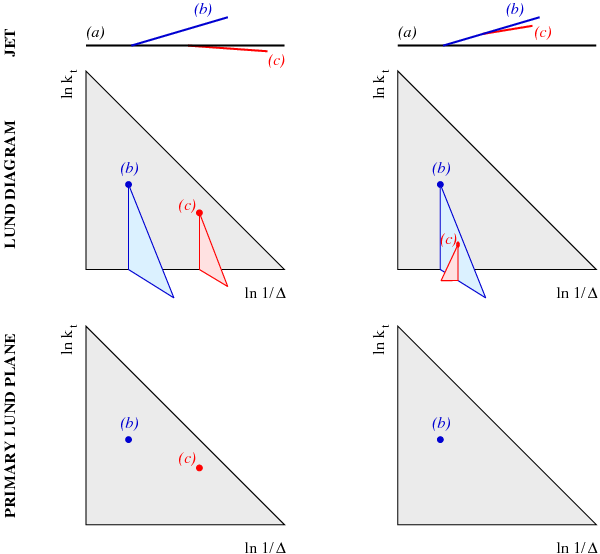
\includegraphics[width=1.0\textwidth]{visuals/figs_lund.png}
\caption{The primary and secondary lund planes for 2 example jets~\cite{Dreyer:2018nbf}.}

\end{figure}


The primary lund plane is shown in Figure ~/ref{fig:lund} ~\cite{Dreyer:2018nbf}
%image 



$P_q(z,\theta^2) dz d \theta^2 = \frac{\alpha_s C_F}{\pi} d( log\frac{1}{z}  ) d(log \frac{1}{ \theta^2})  $\newline

Jets can also be initiated by gluons and this probability is incredibly similar :


$P_q(z,\theta^2) dz d \theta^2 = \frac{\alpha_s C_A}{\pi} d( log\frac{1}{z}  ) d(log \frac{1}{ \theta^2})  $\newline


This similarity allows us to interpret the variations in quark enriched and gluon enriched jet samples in terms of the fundamental $C_F$ and adjoint $C_A$ casimirs, in $SU(3)$ ,   $C_F = \frac{4}{3}$ and $C_A=3$. 


Comparing the probability of a quark to emit a gluon and that of a gluon to to emit a gluon, we can see the ratio is simply $\frac{C_A}{C_F} =\frac{9}{4} $. This has strong experimental implications since it implies gluon jets will on average be composed of about twice as many constituent particles as quark jets.






\section{Event Generation and reconstruction}\label{secMCGenReco}


The events used for this measurement were reconstructed from data aquired by the CMS detector in the case of the data and generated using monte carlo generators PYTHIA and HERWIG in the case of the generated data.

\subsection{Monte Carlo Event Generators}\label{secMCGen}

Monte Carlo (MC) event generators are tools used by both experimental and theoretical physicists to simulate different physical processes in order to make predictions and prepare future experiments. The main tasks of such generators are to calculate matrix elements of the relevant hard processes but they must also describe parton showering, hadronization and underlying event. MC can be utilized to extrapolate data measurements beyond the acceptance of the detector or in the case of this thesis it is used in the unfolding process to correct the data for detector efficiency and resolution.


MC generators provide an ensemble of generated events which realistically describe the theoretical prediction for the physics process in question. Each individual generator implements a slighly different scheme in order to approximate the neccessary calculations for the factorization and renormalization scales relevant to a process. These variations mean that the choice of MC generator will have a slight effect on the generated distributions. For this reason, in the analysis described herein we compared results from 2 different generators: PYTHIA and HERWIG.

PYTHIA is a very commonly used general purpose event generator which uses the parton shower approach for higher order corrections to the hard scattering matrix element.

HERWIG is another commonly used event generator, incredibly similar to PYTHIA, differing mainly in hadronization and parton showering behaviors.


\subsection{Event Reconstruction}\label{secReco}


particle flow


%%%%%%%%%%%% NEW  CHAPTER %%%%%%%%%%%%%%%%%%%%









\chapter{Jets in Proton-Proton Collisions}%\label{ch1:intro}

A jet is a collimated grouping of hadrons usually associated with the production of a parton, quark or gluon, in this case initiated by the hard scatter of 2 constituent partons from protons. The initial parton radiates other quarks and gluons, called the "Parton Shower" and all color charged particles fragment into hardons, mainly pions and kaons,  before reaching the detector.

Studies of jets at LHC are complicated by experimental complexities such as "underlying event", other partons from the same proton iteracting and depoiting energy in the same region of the detector. "Pileup" is also increasingly relevant, like "underlying event" but initiated from other proton interactions from this or a previous bunch since LHC collides $~10^{11}$ protons in bunches every 25 nanoseconds.



Lastly any measurement is limited by the resolution of the measurement device and any detector effects which are disentangled from the signal by "unfolding" the reconstructed distributions back to generator level.

While jets are often used as simple proxies for the quark or gluon from which they originated, the structure of the radiation pattern of the hard scatter is encoded within the jet's constituent particles~\cite{Asquith:2018igt}. Jet studies are essential for a complete understanding of proton-proton interactions since the majority of interesting physics signatures contain a color charged parton in the final state. This chapter covers the basics of jet physics at LHC, from the algorithms used for clustering the constituent particles in experimental data to the language and calculations of the theory.

% cite https://arxiv.org/pdf/1901.10342.pdf simones book



\section{Jet Clustering Algorithms}\label{secSM:ch1}

Ideally, a jet represents a quark [gluon] parton however a more precise definition :

"A phase space region (as defined by an unambiguous
hadronic fiducial cross section measurement) that yields
an enriched sample of quarks [gluons] (as interpreted by some
suitable, though fundamentally ambiguous, criterion)"~\cite{Badger:2016bpw} as defined at the Les Houches confernece in 2015 .

I will discuss one class of "suitable, though fundamentally ambiguous" criteria for defining jets, known as sequential recombination algorithms. These algorithms take pairs of particles and successively combine them into 1 particle, in a way which in intended to reconstruct the successive branchings of partons within the jet as described by perturbative QCD ~\cite{Marzani:2019hun}.
 
In sequential recombination algorithms a distance metric, $d_{ij}$, is defined between all particle pairs, these pairs are then sequentially combined in order of increasing distance.There exist three popular  algorithms in this class, all of the following can be described by the equation ~\cite{Ellis:1993tq}:


\begin{equation}
\begin{array}{l}{d_{i j}=\min \left(p_{t i}^{2 p}, p_{t j}^{2 p}\right) \frac{\Delta R_{i j}^{2}}{R^{2}} \quad \Delta R_{i j}^{2}=\left(y_{i}-y_{j}\right)^{2}+\left(\phi_{i}-\phi_{j}\right)^{2}} \\ {d_{i B}=p_{t i}^{2 p}}\end{array}
\end{equation}


Depending on the value chosen for $p$, this equation can produce a variety of clusterings, herein I discuss the 3 popular choices $p = [1, 0, -1]$ refering to them by their names ; KT ~\cite{Ellis:1993tq}, Cambridge/Aachen ~\cite{Dokshitzer:1997in} and Anti-KT algorithms ~\cite{Cacciari:2008gp}, respectively.








% good section on it here
% http://inspirehep.net/record/1123042/files/fermilab-thesis-2012-12.pdf

%# https://arxiv.org/pdf/1304.1025.pdf
%Sequential recombination algorithm for jet clustering and
KT - > C/A -> Anti-KT
\cite{Tseng:2013dva}



%##image C/A vs anti-Kt --- visuals/config-antikt-double-lund
\begin{figure}[htb]
\centering
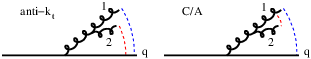
\includegraphics[width=1.0\textwidth]{visuals/config-antikt-double-lund.png}
\caption{How clustering follows radiation pattern for different algorithms~\cite{Dreyer:2018nbf}.}
\label{fig:lund}
\end{figure}

\begin{figure}[htb]
\centering
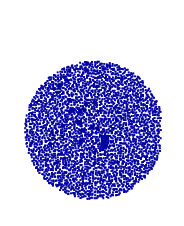
\includegraphics[width=1.0\textwidth]{visuals/figs_subjet-plots-antikt.png}
\caption{How clustering looks for Anti-Kt, circular pattern makes pileup and underlying event subtraction more simple for experimentalists~\cite{Dreyer:2018nbf}.}
\label{fig:lund}
\end{figure}

\begin{figure}[htb]
\centering
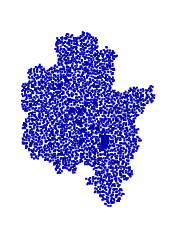
\includegraphics[width=1.0\textwidth]{visuals/figs_subjet-plots-CA.png}
\caption{C/A, not circular, shaped like radiation pattern~\cite{Dreyer:2018nbf}.}
\label{fig:lund}
\end{figure}
%#

%#


\section{Jet Structure}\label{jetstruc:ch1}

The picture is not so simple, we have pileup and underlying event. We analyze the entire radiation pattern and from its structure can determine the probability that a  gluon or quark (even the type of quark) initiated this jet there exist many methods for going about these tasks.

Quark/Gluon discrimination is discussed in section QUARK GLUON SECTION and can be done in many ways such as examining the gluon emission spectrum as visualized in the lund plane as mentioned in the introduction. In this section quark jet discrimination is discussed, specifically how the higher order corrections to the hard process are nessessary in order to properly predict measurements in the non-perturbative regime.

NLO + NLL + NP to match data in non-perturbative regime

\begin{figure}[htb]
\centering
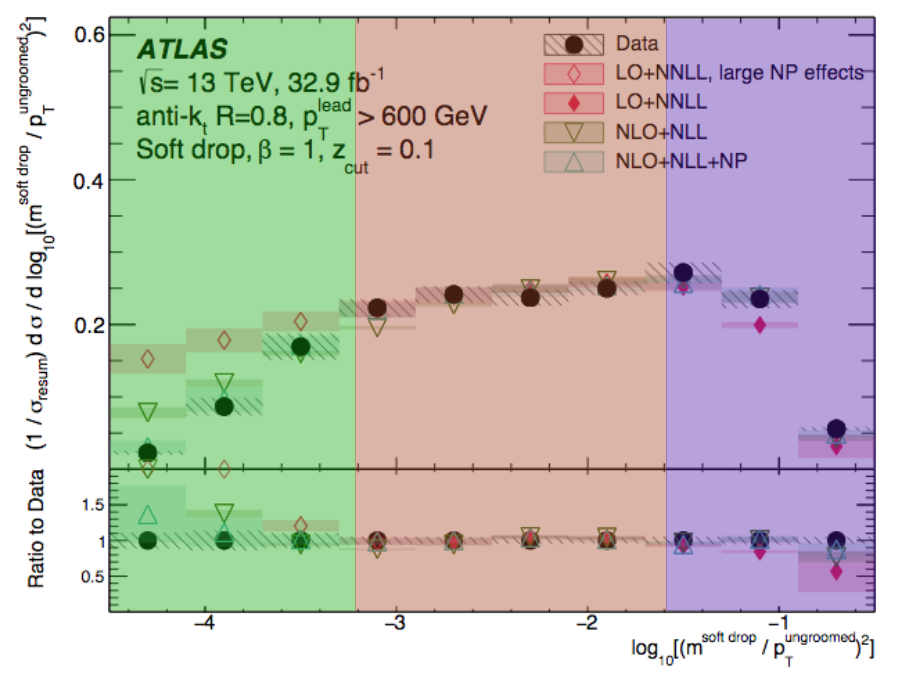
\includegraphics[width=1.0\textwidth]{visuals/ATLAS-rho-highorder.png}
\caption{ATLS DIJets Rho result~\cite{Dreyer:2018nbf}.}
\label{fig:lund}
\end{figure}



% pilup images with diff algorithms
%# https://arxiv.org/pdf/1304.1025.pdf
%Sequential recombination algorithm for jet clustering and

%Towards Jetography
%Gavin P. Salam
%$https://arxiv.org/abs/0906.1833
\cite{Salam:2009jx}

\cite{Asquith:2018igt}
%https://arxiv.org/pdf/1803.06991.pdf
%Jet Substructure at the Large HadronCollider :  Experimental Review

\section{Jet Grooming}\label{jetgroom:ch1}

Soft-drop

other grooomers

image of soft drop compared to others

image of soft drop grooming tree


%Casimir Meets Poisson: Improved Quark/Gluon Discrimination with Counting Observables
%https://arxiv.org/abs/1704.06266
%soft drop multiplicity



% DY thesis https://cds.cern.ch/record/2018454/files/CERN-THESIS-2015-048.pdf
\section{Jet Production Cross Sections}\label{jetgroom:ch1}



\begin{equation}
\sigma=\sum_{a, b} \int_{0}^{1} d x_{a} d x_{b} \int d \Phi_{n} f_{a}^{h_{1}}\left(x_{a}, \mu_{F}\right) f_{b}^{h_{2}}\left(x_{b}, \mu_{F}\right) \frac{1}{2 \hat{s}}\left|\mathcal{M}_{a b \rightarrow n}\right|^{2}\left(\Phi_{n} ; \mu_{F}, \mu_{R}\right)
\end{equation}



